\documentclass[11pt,letterpaper]{article}

\usepackage[utf8]{inputenc}
\usepackage[spanish]{babel}
\usepackage{float}
\usepackage{xcolor}
\usepackage{verbatim}
\usepackage{mwe}
\usepackage{charter}
\usepackage{afterpage}
\usepackage{amsmath}
\usepackage{appendix}
\usepackage{ragged2e}
\usepackage{array}
\usepackage{etoolbox}
\usepackage{fancyhdr}
\usepackage{booktabs}
\usepackage{arydshln}
\usepackage[justification=justified,singlelinecheck=false,labelfont=bf,format=plain]{caption}
\usepackage[justification=justified,singlelinecheck=false,labelfont=bf,format=plain]{subcaption}
\usepackage{enumitem}
\usepackage[bottom=2.5cm,top=2.0cm,left=2.0cm,right=2.0cm]{geometry}
\usepackage{graphicx}
\usepackage{indentfirst}
\usepackage{mathtools}
\usepackage{multirow}
\usepackage{pdfpages}

\usepackage{subfiles}
\usepackage[compact]{titlesec}
\usepackage{blindtext}
\usepackage{stfloats}
\usepackage{lipsum} 


\renewcommand{\familydefault}{\rmdefault}

\newcommand\blankpage{
    \null
    \thispagestyle{empty}
    \addtocounter{page}{0}
    \newpage}

\newcolumntype{L}[1]{>{\raggedright\let\newline\\arraybackslash\hspace{0pt}}m{#1}}
\newcolumntype{C}[1]{>{\centering\let\newline\\arraybackslash\hspace{0pt}}m{#1}}
\newcolumntype{R}[1]{>{\raggedleft\let\newline\\arraybackslash\hspace{0pt}}m{#1}}

    \setlist[itemize,1]{label=$\bullet$}
    \setlist[itemize,2]{label=$\circ$}
    \setlist[itemize,3]{label=$-$}
    \setlist{nosep}
    \title{Circuito RL con salida en R}
    \author{Álvaro Martín Romero}
    
    
\begin{document}
\maketitle
\section{Cálculos del circuito de forma teórica}%
\label{sec:Ejercicio 1}
Analizaremos en este ejercicio el circuito RL con salida en R de forma teórica, calculando primero la función de transferencia.\\
\\
Para ello, sabemos que la función de transferencia en función de la variable $s$ vale:
\[
	G(s)=\frac{V_s(s)}{V_e(s)}
.\] 
Donde $V_s(s)$ y $V_e(s)$ son las tensiones de salida y entrada respectivamente. Sustituyendo según sus definiciones:
\[
	V_s(s)=I\cdot R; \\ \\ \\ \\  \\ V_e(s)=I\left( R+LS \right) 
.\] 
en la función de transferencia, nos da el módulo de la función de transferencia:
\[
	G(jw)=\frac{1}{1+ j\omega T}
.\] 
Siendo $T=\frac{L}{R}$ \\
\\

La frecuencia de corte se define como el límite en la respuesta frecuencial de un circuito en el cual la energía que fluye a través de él empieza a atenuarse. La frecuencia de corte se define como:
\[
f_c=\frac{w_c}{2\pi}
.\] 
siendo $w_c= \frac{1}{T}$, o lo que es lo mismo $w_c=\frac{R}{L}$. Sustituyendo nuestros datos dados en el enunciado $\left( R=10 k\Omega, L=350mH \right) $ nos da una frecuencia de corte de :

\begin{equation}
f_c= 4547.28 Hz
\end{equation}
El ejercicio nos pide el desfase y el valor teórico de la tensión de salida para el valor de la frecuencia igual que la frecuencia de corte. Estos valores son:
\begin{equation}
	\boxed{	\theta= -\arctan \left( \frac{w}{w_c} \right) =-\arctan(1)=-\frac{\pi}{4}=-45º}
\end{equation}
El valor de la tensión de salida se define como:
\[
	V_s(s)= \mid G(jw) \mid \cdot V_e(s)
.\]
donde $V_e(s)$  es $20 Vpp$ y  $ \mid G(jw) \mid =\frac{1}{\sqrt{1+\left( \omega\cdot T \right) ^2}}$. Por tanto:
\begin{equation}
	\boxed{V_s(s)=\frac{1}{1+\left( \omega\cdot T \right) ^2}\cdot 10=\frac{10}{\sqrt{2} }=7.07 V}
\end{equation}
En este ejercicio también nos piden calcular la tensión de salida y el ángulo de desfase para una década por encima y por debajo de la frecuencia de corte. Para ello haremos lo mismo pero para un $w_c$ una década por encima (es decir, multiplicar por 10) y una década por debajo (multiplicar por 0,1):\\
\\
Para una década por encima:\\
\\
La nueva $\omega$ se define como $\omega=10\cdot \omega_c$, siendo $w_c=28571.42$ los valores que nos piden son:
\begin{equation}
	\boxed{\theta= -\arctan\left( \frac{\omega}{\omega_c} \right) = -\arctan\left( \frac{285714.2}{28571.42} \right) =-84.28º}
\end{equation}
\begin{equation}
\boxed{V_s\left( s \right) = \mid G(jw) \mid \cdot V_e(s)=\frac{1}{\sqrt{1+\left( \frac{w}{w_c} \right)^2}} \cdot 10= 0.9950 V}
\end{equation}
Para una década por debajo:\\
\\
$\omega=0.1\cdot \omega_c= 2857.142$:

\begin{equation}
	\boxed{\theta=-\arctan \left( \frac{\omega}{\omega_c} \right) =-5.71}
\end{equation}
 \begin{equation}
	 \boxed{V_s\left( s \right) = 9.95 V}
\end{equation}

\section{Circuito en el simulador con análisis AC}%
\label{sec:Circuito en el simulador con análisis AC}

A continuación comprobaremos los valores teóricos obtenidos anteriormente mediante el programa MultisimLive. Para ello mostramos en pantalla el circuito hecho mediante este simulador:
\begin{figure}[h]
	\centering
	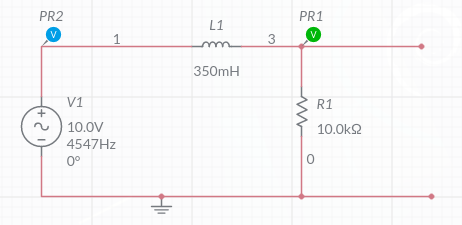
\includegraphics[width=0.6\textwidth]{imagen/circuitoRL_R.png}
	\centering{\caption{Muestra del circuito RL con salida en R hecho en MultisimLive}}
\end{figure}
Mediante el gráfico que nos proporciona el programa podemos ver las tensiones de salida y de entrada gracias a los cursores situados en los picos:
\begin{figure}[H]
	\centering
	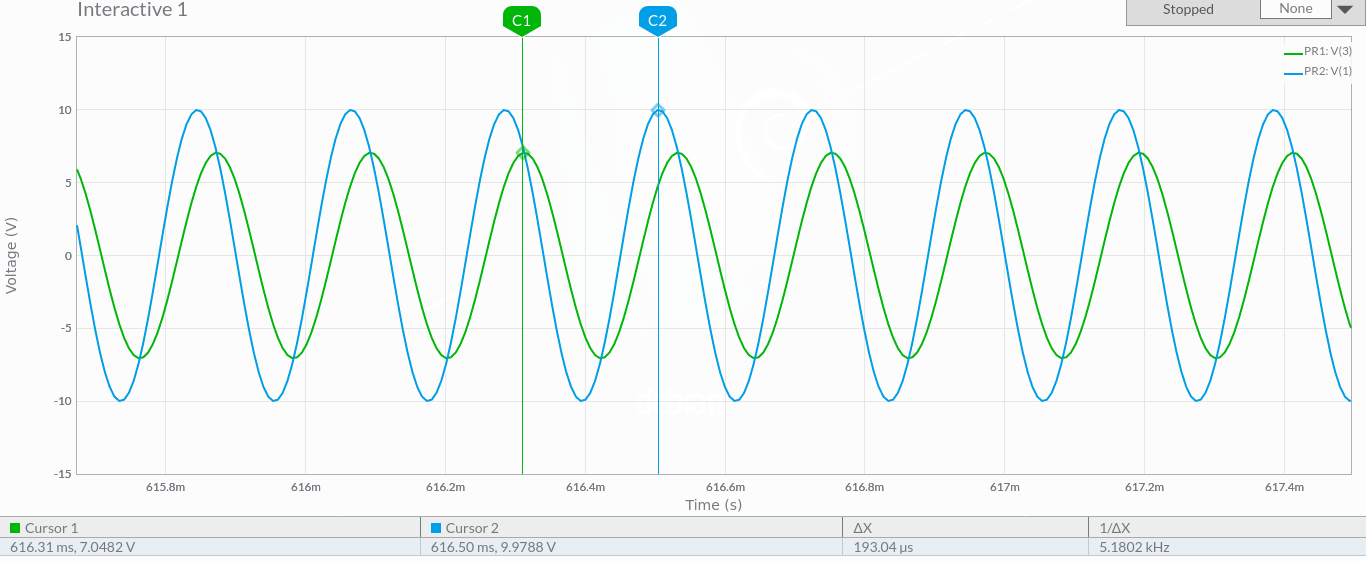
\includegraphics[width=0.8\textwidth]{imagen/analisispotenciales.png}
	\label{fig:analisispotencial-png}
	\caption{Análisis de tensión de salida y entrada con la gráfica de MultisimLive}
\end{figure}
Como vemos, los resultados para el resultado del valor de la tensión de entrada coincide con el resultado teórico. Aunque este valor no es del todo exacto debido a que el programa tiene cierta sensibilidad a la hora de medir exactamente el pico de la curva de tensión.\\
\\
Ahora realizaremos otro análisis para hallar la frecuencia de g¡corte gracias a la gráfica del análisis AC:
\begin{figure}[H]
	\centering
	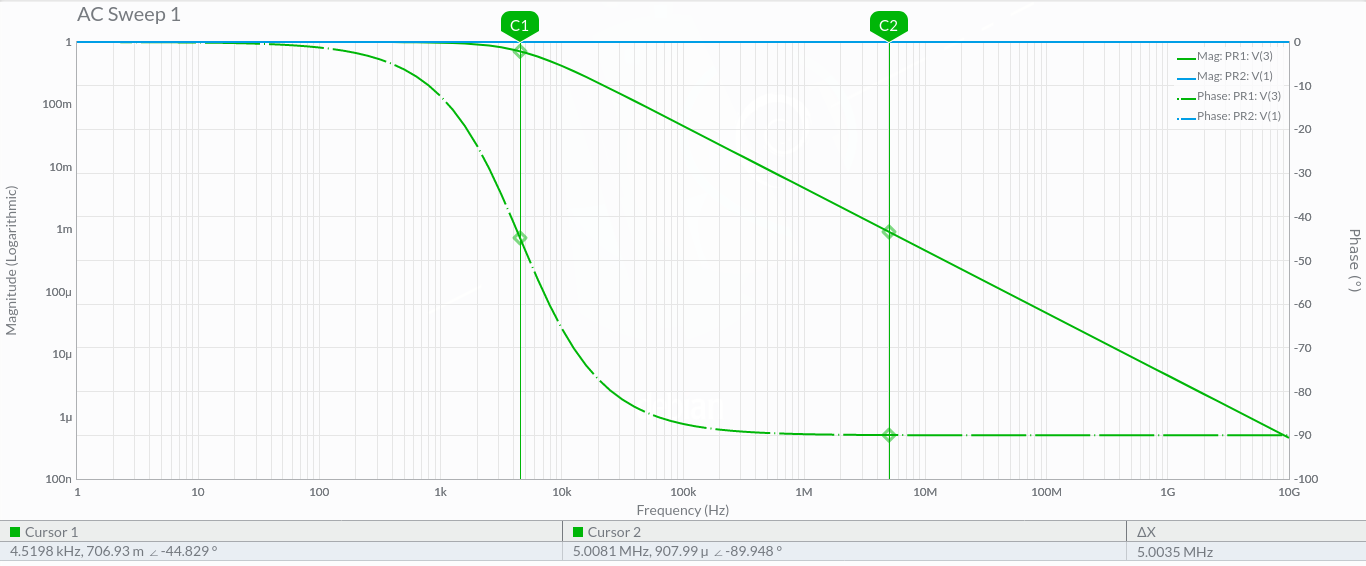
\includegraphics[width=0.8\textwidth]{imagen/analisisAC.png}
	\caption{Representación AC Sweep para hallar la frecuencia de corte}
	\label{fig:imagen-analisisAC-png}
\end{figure}
En la figura vemos que la frecuencia para el ángulo $\theta=45º$ es aproximadamente la frecuencia de corte que medimos de forma teórica.\\
\\
Nos queda representar el circuito para una frecuencia una década arriba y abajo de la de corte. Podemos variar uno de los parámetros que definen la frecuencia para que nos dé el valor que queramos. Los resultados gráficos son:
\begin{figure}[H]
	\centering
	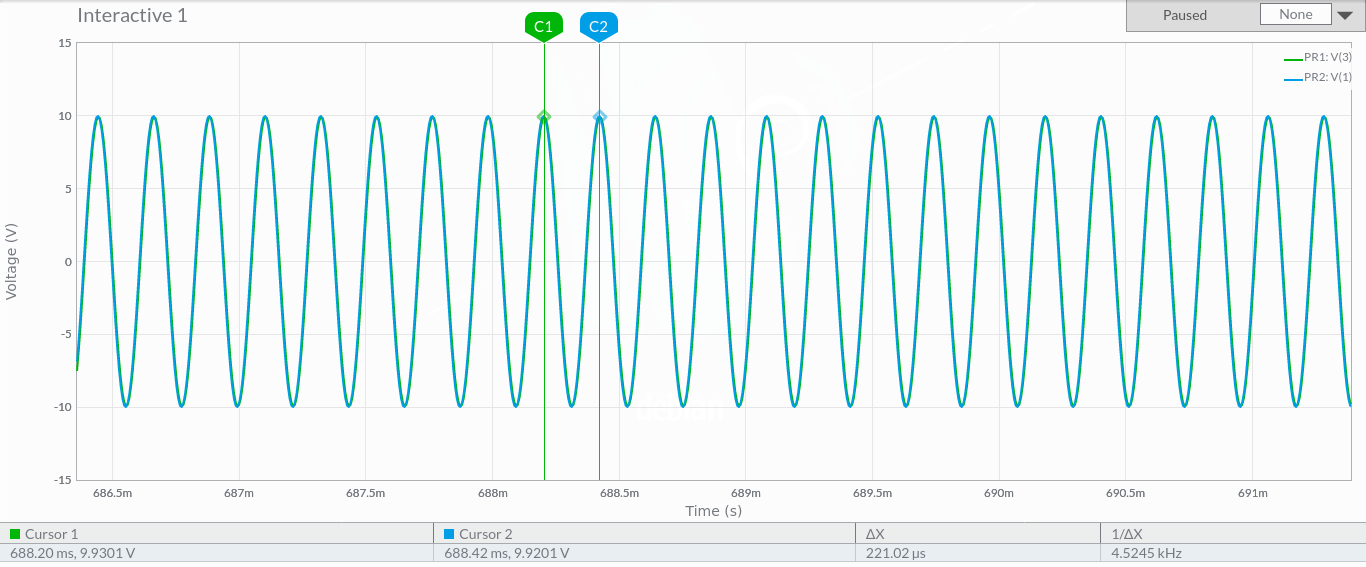
\includegraphics[width=0.8\textwidth]{imagen/decadaarriba.png}
	\caption{Cálculo gráfico de la tensión de salida para una década por encima de la frecuencia de corte}
	\label{fig:imagen-decadaarriba-png}
\end{figure}
Como vemos en el cursor de la función en color verde, el valor dela tensión de salida es aproximadamente el valor teórico obtenido anteriormente, tal como cabría esperar. Haremos lo mismo para una década por debajo de la frecuencia de corte:
\begin{figure}[H]
	\centering
	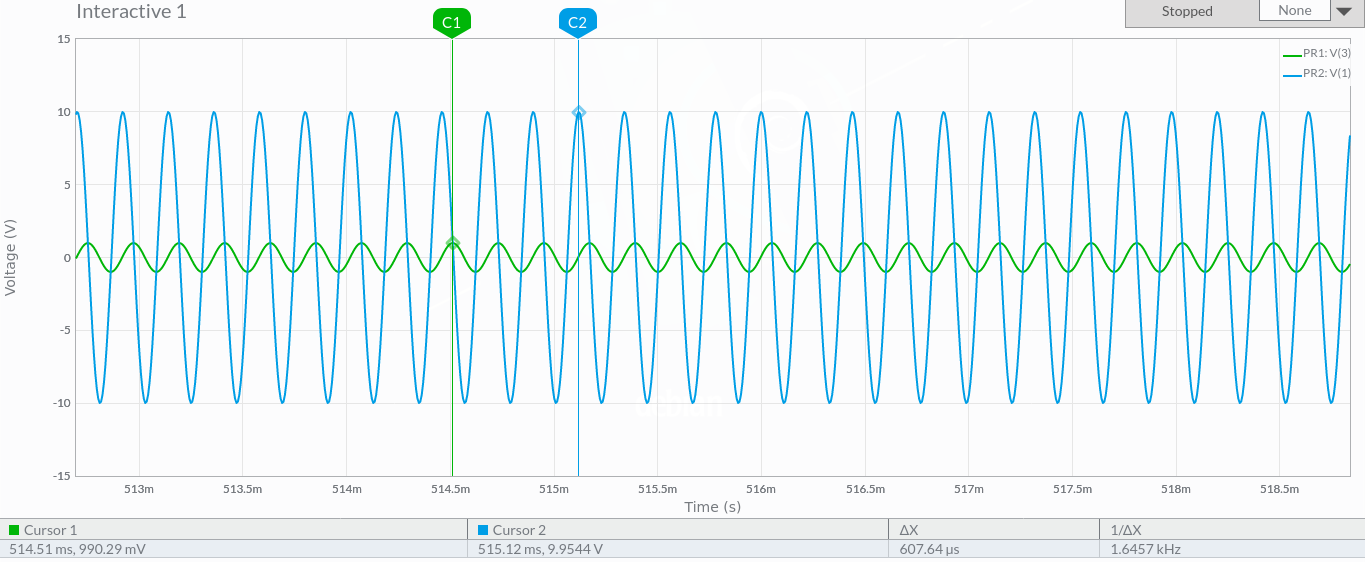
\includegraphics[width=0.8\textwidth]{imagen/decadaabajo.png}
	\caption{Cálculo gráfico de la tensión de salida para una década por debajo de la frecuencia de corte}
	\label{fig:}
\end{figure}
A continuación vamos a representar gráficamente para ver el valor de la frecuencia una década por encima y por debajo de la frecuencia de corte mediante la gráfica AC Sweep:
\begin{figure}[H]
	\centering
	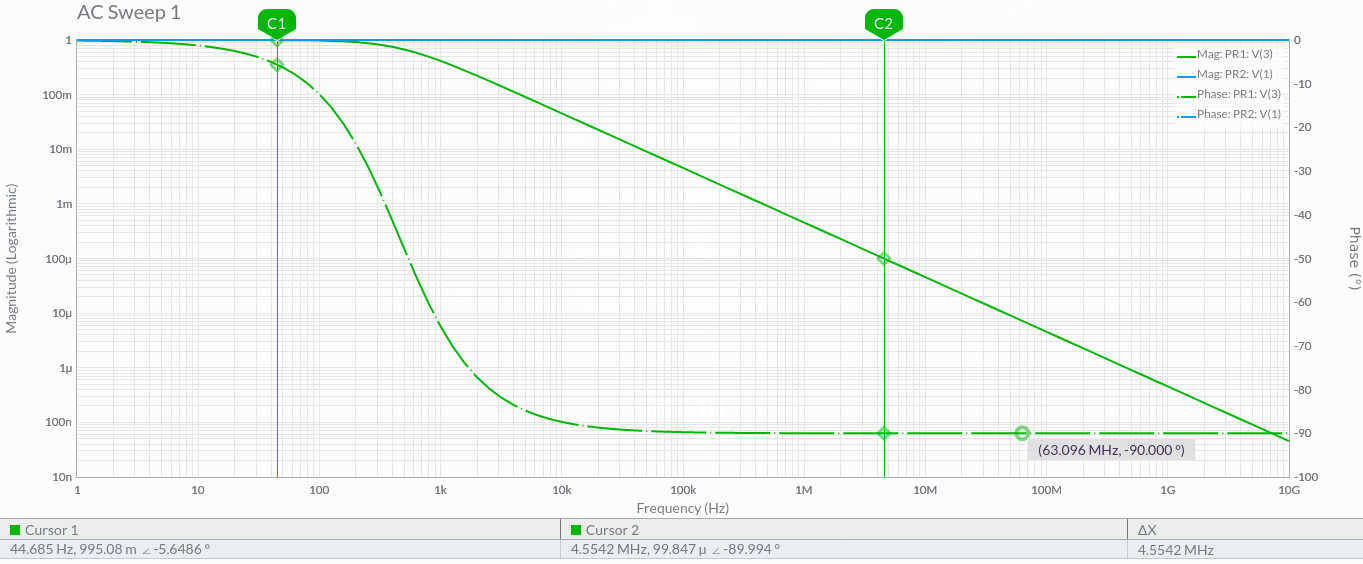
\includegraphics[width=1\textwidth]{imagen/accorte.png}
	\caption{Representación gráfica AC para ver la frecuencia una década por encima y por debajo de la frecuencia de corte}
	\label{fig:imagen-accorte-png}
\end{figure}
Se puede ver que los valores del desfase concuerdan con los valores teóricos obtenidos, siendo el cursor C1 para una década inferior y C2 para una superior

\section{Conclusiones del comportamiento del circuito}%
\label{sec:Conclusiones del comportamiento del circuito}
El comportamiento del circuito lo podemos observar al medir las características de este cuando la frecuencia es diferente a la frecuencia de corte. \\
\\
Cuando esta frecuencia es baja (una década por debajo) observamos que el desfase es ínfimo, casi despreciable frente al desfase cuando la frecuencia es la de corte. Por consiguiente, el voltaje de salida es muy parecido al de entrada.\\
\\
Por contraposición, cuando la frecuencia es una década más alta que la de corte, el desfase se hace muy alto y la respuesta del voltaje de salida del circuito es mucho menor que el de entrada.\\
\\
Podemos decir por tanto que el filtro del circuito se encarga de despreciar las frecuencias mayores que la de corte y permite que las frecuencias más bajas pasen por el. 
\end{document}


